\subsection{Functional Role}

In order to simply the comprehension of the functional role of the class to be inspect, a brief explanation of the context where the class is placed is given.

\paragraph{The OFBIz's: Overview}
The Open For Business project is an enterprise-oriented suite of applications developed to support most of the aspects that an enterprise application has to take care of.
The applications share the same underlying architecture, using common data, logic and process components.
Each application is loosely coupled with the others, easing the updating and the extension.

% 22 minuti

\paragraph{The Components:}

The architecture of the entire suite is composed by 4 sets of components:
\begin{itemize}
	\item \textbf{Framework}
	\item \textbf{Applications}
	\item \textbf{Special Purpose}
	\item \textbf{Hot-deploy}
\end{itemize}

The sets of components are in relation according to the dependency-arcs shown in the following diagram.
The relationship hierarchy goes from top to bottom, meaning that components and applications on the top are dependent on elements on the bottom of the same diagram.

\begin{figure}[H]
	\centerline{
		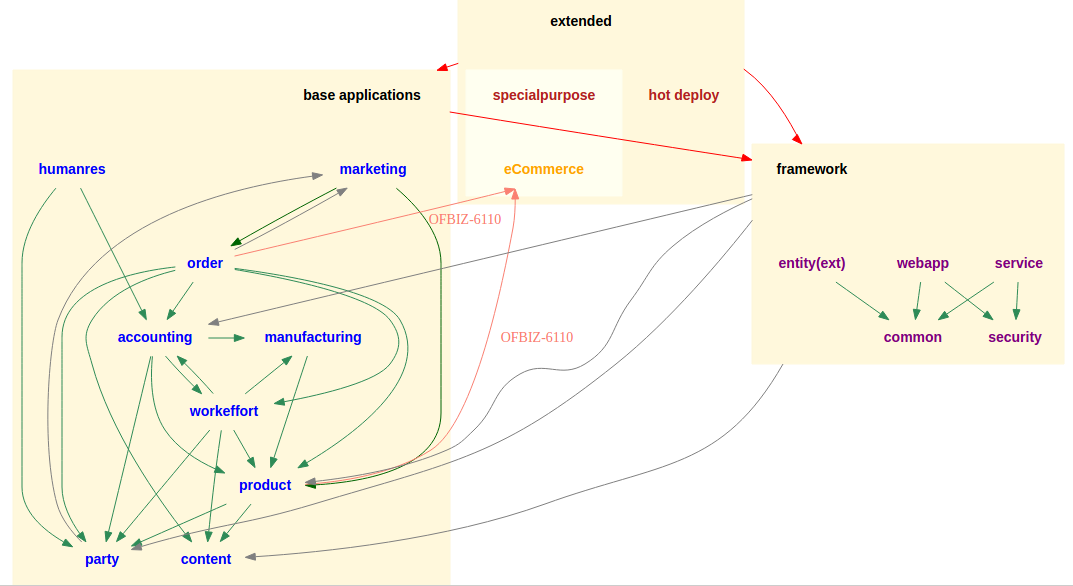
\includegraphics[width=350px]{../Datas/images/dependencies.png}
	}
\end{figure}

\paragraph{The party:}
Before going to the main topic of this section, that is the functional role covered by the human resource java class, a glance to this aspect of the system is worthful since it's a dependecy of human resource application and since it's quite recurrent in the human resource.

According to the \href{https://ofbiz.apache.org/apache-ofbiz-project-overview.html}{\textit{OFBIz project overview}}:

Party can be either a Person, or a group of Parties. A Party Group could be a company, an organization within the company, a supplier, a customer, and so forth. Information that describes Parties or is directly related to Parties is contained in these entities.

\paragraph{The role of the human resources application:}

According to the \href{https://ofbiz.apache.org/apache-ofbiz-project-overview.html}{\textit{OFBIz project overview}}:

The Human Resources entities are used to keep track of positions, responsibilities, skills, employment, termination, benefits, training, pay grades and payroll preferences, performance reviews, resumes and applications, and other Human Resources related information.

According to the \textit{HELP\_HR.XML} file, located in the \textit{data/helpdata} folder of the \textit{humanres} application, the humar resource aplication is developed in order to provide a solid and extensible backbone for the development of such a platform.

Always according to this file, the application backbone may provide a \textit{tree reporting structure} showing the parties positions in the companies.

% TREE STRUCTURE:
% + COMPANY
%  |_ DEP1
%   |~EMPL1
%   |~EMPL2
%   ||_ DEP2
%    ||~EMPL3
%    ||~EMPL4
%   ||_DEP3
Of particular interest is the file \textit{HELP\_HR\_main.XML}, located in the same folder of the previously cited xml file, where the main screen of the application is described. As stated in this file:

The Main window is the entry point into the Human Resources Application and displays the Company tree view for navigating to the main menu items.

Always according to this file:

There are three node types in the tree, each identified by a different icon. 
The top of the tree represents your Company, the highest level in the organization. The Company and departments under the Company can have sub departments or positions.
Under positions are the people who fulfill the position.

Always according to this file, the main screen allows:

\begin{itemize}
	\item The navigation of the company hierarchy, viewing departements, position and people.
	\item Add or remove a department
	\item Add a person
	\item Quickly open the profile of any item in the tree
	\item If an item is a position, you can add a person to fulfill the position.
\end{itemize}

After this brief analysis of the context where the human resource application lives and the functionalities provided, we can analyze the role of the class given us, dissecting each of its method.

\paragraph{HumanResEvents class: overview}:

This class is supposed to support all the functionalities that the humanres application backbone has to provide. This has been already listed in the previous paragraph.

Up to these release, the class presents 4 methods: one public and the rest private.
The private methods are used as helper functions by the public one.

In the following the methods composing the class are described in details.

\paragraph{getChildHRCategoryTree:}

Only public method exposed by the HumanResEvents class. It's functional role is to manage the request of visualization of a given node of the tree describing the enterprise hierarchy.

The method retrieves the informations regarding the child requested. This, according to the party definition, may be an employee or the company or a department (partyGroup).

If the former is the case, the informations of the employee selected are returned. If the latter is the case, the departments that are child of the department selected or of the company, in the case the root of the tree has been selected, are returned, along with the informations about the employees that work in the selected department or company

% This can be infered both from the informations in the xml files presented before and the few comments in the method.


\paragraph{getCurrentEmployeeDetails:}

Helper method used to retrieve the information of a given employee.
It first checks if the given partyID has 
The informations retrieved are the Name and Surnamen of the employee.


% l.107: maybe this is done by l.101

% 1h 38min
%Explain the context of the human resource app and role
% Explain how the human resource informations are structured
% e.g.: tree structure
% HELP_HR_main

% Explain what is a party and the relation with the humanres
% https://cwiki.apache.org/confluence/display/OFBIZ/Component+and+Component+Set+Dependencies
% https://ofbiz.apache.org/apache-ofbiz-project-overview.html

% The variables "ctx" and "ctxs" are used as "context" abbreviations
